\documentclass[12pt,a4paper]{article}

% ─── Core Packages ───────────────────────────────────────────────────────────
\usepackage[margin=1in]{geometry}
\usepackage[T1]{fontenc}
\usepackage{lmodern}
\usepackage{amsmath,amssymb,amsthm}
\usepackage{mathtools}
\usepackage{graphicx}
\usepackage{xcolor}
\usepackage{booktabs}
\usepackage{multirow}
\usepackage{array}
\usepackage{enumitem}
\usepackage{algorithm}
\usepackage{algpseudocode}
\usepackage{tcolorbox}
\usepackage{microtype}
\usepackage{caption}
\usepackage{natbib}
\usepackage{tikz}
\usepackage{pgfplots}
\pgfplotsset{compat=1.18}
\usetikzlibrary{positioning,arrows.meta,shapes.geometric,fit}
\usepackage{listings}
% ─── hyperref and cleveref must come last ────────────────────────────────────
\usepackage{hyperref}
\usepackage[noabbrev]{cleveref}

% ─── Color Definitions ───────────────────────────────────────────────────────
\definecolor{intuitionbg}{RGB}{235,245,255}
\definecolor{intuitionborder}{RGB}{70,130,200}
\definecolor{mathbg}{RGB}{245,240,255}
\definecolor{mathborder}{RGB}{130,70,200}
\definecolor{warnbg}{RGB}{255,245,235}
\definecolor{warnborder}{RGB}{200,130,70}
\definecolor{implbg}{RGB}{235,255,240}
\definecolor{implborder}{RGB}{70,180,100}
\definecolor{codegray}{RGB}{245,245,245}
\definecolor{codekey}{RGB}{0,0,180}
\definecolor{codecomment}{RGB}{100,100,100}
\definecolor{codestring}{RGB}{160,32,32}

% ─── Listings Setup (replaces verbatim) ──────────────────────────────────────
\lstset{
  language=Python,
  basicstyle=\ttfamily\small,
  keywordstyle=\color{codekey}\bfseries,
  commentstyle=\color{codecomment}\itshape,
  stringstyle=\color{codestring},
  backgroundcolor=\color{codegray},
  frame=single,
  framerule=0.4pt,
  rulecolor=\color{gray!40},
  numbers=left,
  numberstyle=\tiny\color{gray},
  numbersep=6pt,
  breaklines=true,
  showstringspaces=false,
  tabsize=2,
  xleftmargin=12pt,
  xrightmargin=4pt,
}

% ─── tcolorbox Environments ──────────────────────────────────────────────────
\tcbuselibrary{skins,breakable}

\newtcolorbox{intuitionbox}[1][]{
  enhanced, breakable,
  colback=intuitionbg, colframe=intuitionborder,
  fonttitle=\bfseries\small, title={Intuition},
  left=6pt, right=6pt, top=4pt, bottom=4pt,
  arc=4pt, #1}

\newtcolorbox{mathbox}[1][]{
  enhanced, breakable,
  colback=mathbg, colframe=mathborder,
  fonttitle=\bfseries\small, title={Formal Definition},
  left=6pt, right=6pt, top=4pt, bottom=4pt,
  arc=4pt, #1}

\newtcolorbox{warnbox}[1][]{
  enhanced, breakable,
  colback=warnbg, colframe=warnborder,
  fonttitle=\bfseries\small, title={Failure Mode},
  left=6pt, right=6pt, top=4pt, bottom=4pt,
  arc=4pt, #1}

\newtcolorbox{implbox}[1][]{
  enhanced, breakable,
  colback=implbg, colframe=implborder,
  fonttitle=\bfseries\small, title={Implementation Note},
  left=6pt, right=6pt, top=4pt, bottom=4pt,
  arc=4pt, #1}

% ─── Math Operators ──────────────────────────────────────────────────────────
\DeclareMathOperator*{\argmin}{arg\,min}
\DeclareMathOperator*{\argmax}{arg\,max}
\DeclareMathOperator{\Softmax}{Softmax}
\DeclareMathOperator{\TopK}{TopK}
\DeclareMathOperator{\Concat}{Concat}
\DeclareMathOperator{\Upsample}{Upsample}
\DeclareMathOperator{\reshape}{reshape}
\DeclareMathOperator{\flatten}{flatten}
\DeclareMathOperator{\IoU}{IoU}
\DeclareMathOperator{\simop}{sim}

% ─── Math Shorthands (conflict-free names) ───────────────────────────────────
% NOTE: \bm is NOT redefined — it would conflict with the bm package.
% We use explicit \mathbf{} or these aliases instead.
\newcommand{\R}{\mathbb{R}}
\newcommand{\E}{\mathbb{E}}
\newcommand{\vv}{\mathbf{v}}     % visual token vector
\newcommand{\vq}{\mathbf{q}}     % query vector
\newcommand{\vm}{\mathbf{m}}     % mask vector  (was \bm — conflict fixed)
\newcommand{\vs}{\mathbf{s}}     % score vector
\newcommand{\mI}{\mathbf{I}}     % image matrix
\newcommand{\mQ}{\mathbf{Q}}     % query sequence
\newcommand{\mV}{\mathbf{V}}     % visual token matrix

% ─── Theorem Environments ────────────────────────────────────────────────────
\newtheorem{proposition}{Proposition}
\newtheorem{remark}{Remark}
\newtheorem{definition}{Definition}

% ─── Hyperref Setup ──────────────────────────────────────────────────────────
\hypersetup{
  colorlinks=true,
  linkcolor=mathborder,
  citecolor=implborder,
  urlcolor=intuitionborder,
  pdftitle={TC-ViTok: Task-Conditioned Visual Tokenization},
  pdfauthor={Muhammad Ali Shah and Talha Hassan Ul Haq}
}

% ════════════════════════════════════════════════════════════════════════════
\begin{document}
% ════════════════════════════════════════════════════════════════════════════

\title{
  \textbf{TC-ViTok: Task-Conditioned Visual Tokenizer} \\
  \large Learning a Token Selection Policy for Efficient Vision-Language Reasoning \\[0.5em]
  \normalsize A Research Paper and Technical Tutorial
}

\author{
  Muhammad Ali Shah \and Talha Hassan Ul Haq \\[0.3em]
  Lahore University of Management Sciences (LUMS) \\
  \texttt{\{27100172, 27100306\}@lums.edu.pk}
}

\date{\today}

\maketitle
\thispagestyle{empty}

% ────────────────────────────────────────────────────────────────────────────
\begin{abstract}
% ────────────────────────────────────────────────────────────────────────────

Vision-language models (VLMs) such as LLaVA process a \emph{fixed} set of $N$
visual tokens regardless of the complexity or spatial specificity of the language
query. This is fundamentally wasteful: a question such as ``What is written on
the sign?'' requires high-resolution attention to one small region, while ``Is
there a cat in this image?'' requires only coarse global features. We introduce
\textbf{TC-ViTok} (Task-Conditioned Visual Tokenizer), a lightweight module that
\emph{learns a token selection policy} $\pi\colon (\mQ, \mI_{\mathrm{coarse}})
\to \mathcal{S}$ mapping a language query and a coarse image representation to a
sparse subset $\mathcal{S}$ of $k \ll N$ visual tokens. Using a 3M-parameter
cross-attention policy network (TPN) and a DINOv2-S coarse encoder, TC-ViTok
conditions the tokenization decision on the language query before the selected
tokens enter the full visual encoder. Unlike existing compression methods, which
are query-agnostic, TC-ViTok predicts task-relevant spatial regions and allocates
the visual token budget accordingly. The policy is trained end-to-end via a
Gumbel-Sigmoid straight-through estimator with a phased training curriculum and
compression regularization to avoid degenerate solutions. We evaluate on VQAv2,
GQA, and TextVQA, showing that query-conditioning provides selective improvements
concentrated in spatially-grounded questions---the precise regime where fixed-budget
tokenization is most harmful---while using $4\times$ fewer visual tokens on average.

\end{abstract}

\tableofcontents
\newpage

% ════════════════════════════════════════════════════════════════════════════
\section{Introduction}
\label{sec:intro}
% ════════════════════════════════════════════════════════════════════════════

\subsection{The Problem: Fixed-Budget Visual Processing}

Modern VLMs encode images into a fixed sequence of $N$ visual tokens, each
corresponding to a patch of the input image. LLaVA-1.5~\citep{liu2024llava}
produces $N = 576$ tokens from a $336 \times 336$ image using a $14 \times 14$
patch size. These tokens are concatenated with text tokens and passed to a large
language model (LLM) whose prefill cost scales as $\mathcal{O}(N \cdot (N + L)
+ L^2)$ for a causal attention LLM with $N$ visual prefix tokens and $L$ text
tokens, where visual tokens attend to each other and text tokens attend to visual
tokens. For typical queries ($L \approx 30$), visual tokens dominate the
attention computation by an order of magnitude.

The fundamental mismatch is this: \textbf{the number of visual tokens is
determined by image resolution, not by task difficulty or spatial locality}.
Every query---whether it requires localised fine-grained reading or global scene
understanding---receives the same 576-token visual budget. This is structurally
analogous to allocating the same number of words to describe every photograph in
a caption task, regardless of whether the image is a blank wall or a crowded
marketplace.

\subsection{Why Existing Solutions Fall Short}

Several approaches attempt to reduce the visual token count:

\begin{itemize}[leftmargin=2em]
  \item \textbf{Token Merging (ToMe)}~\citep{bolya2022token}: Merges visually
    similar tokens inside the ViT using bipartite soft matching. The merging
    criterion is embedding-space similarity---purely image-driven, entirely
    query-agnostic.
  \item \textbf{LLaVA-PruMerge}~\citep{shang2024llava}: Prunes visual tokens
    based on their cross-attention weight with the [CLS] token. This summarises
    the \emph{whole image}, not the query. The full ViT forward pass also runs
    first; compute is only saved in the LLM, not the ViT.
  \item \textbf{DynamicViT}~\citep{rao2021dynamicvit}: Learns to drop tokens
    inside the ViT using a prediction network. This is content-adaptive but not
    conditioned on any external query signal.
\end{itemize}

The shared limitation of all existing methods is that \textbf{the compression
decision is made without knowledge of the task}. They learn which visual tokens
are generally important, not which tokens are important \emph{for this specific
question}.

\subsection{Our Approach: Tokenization as a Policy}

We propose a conceptual shift: \textbf{visual tokenization should be treated as
a learned policy, not a fixed procedure}. A policy takes as input the task
specification (the language query) and a representation of the image, and outputs
a computational action (the selected token set). We seek a function
\[
  \pi\colon (\mQ,\, \mI_{\mathrm{coarse}}) \;\longrightarrow\; \mathcal{S}
    \;\subseteq\; \{1, \ldots, N\}, \quad |\mathcal{S}| = k
\]
that selects $k$ out of $N$ tokens conditioned jointly on the query and the
image. Unlike a representation (which produces an embedding) or an attention
bias (which reweights existing computation), a policy governs \emph{which
computation is performed} upstream of the main model.

\subsection{Contributions}

This work makes the following contributions:

\begin{enumerate}[leftmargin=2em]
  \item \textbf{Conceptual:} We formalise visual tokenization as a
    query-conditioned discrete policy problem, providing the first systematic
    study of this framing.
  \item \textbf{Architectural:} We introduce the Tokenization Policy Network
    (TPN), a lightweight ($\approx 3$M parameter) cross-attention module that
    produces spatial token-selection masks conditioned on language queries.
  \item \textbf{Training:} We propose a phased training curriculum with
    Gumbel-Sigmoid annealing and compression regularization that avoids the
    degenerate solutions that otherwise dominate training.
  \item \textbf{Analytical:} We introduce a \emph{spatial specificity evaluation
    protocol} that stratifies VQA questions by their dependence on localised
    visual evidence, enabling fine-grained hypothesis testing.
\end{enumerate}

% ════════════════════════════════════════════════════════════════════════════
\section{Related Work}
\label{sec:related}
% ════════════════════════════════════════════════════════════════════════════

\subsection{Vision-Language Models}

Large VLMs have converged on a recipe: a visual encoder (typically a CLIP
ViT~\citep{radford2021learning}), a projection layer, and a frozen or
instruction-tuned LLM~\citep{liu2024llava,li2023blip2,bai2023qwenvl}. LLaVA-1.5
\citep{liu2024llava} established a clean baseline with a two-layer MLP projector
and Vicuna-7B. Subsequent work (LLaVA-1.6, LLaVA-HR) increases resolution via
image tiling, generating 2880+ visual tokens---exacerbating the efficiency
problem we address. Our work builds directly on LLaVA-1.5 as the backbone.

\subsection{Visual Token Compression}

Token compression methods fall into two categories. \emph{Within-ViT} methods
(ToMe~\citep{bolya2022token}, DynamicViT~\citep{rao2021dynamicvit},
EViT~\citep{liang2022evit}) reduce tokens during the ViT's forward pass using
similarity-based or attention-based criteria---all query-agnostic. \emph{Post-ViT}
methods (LLaVA-PruMerge~\citep{shang2024llava}, FastV, LLaVA-UHD) apply
compression after the ViT outputs embeddings, saving only LLM context cost.
TC-ViTok is the first method to condition the compression decision on the
language query, and applies the mask decision before full token processing
where possible.

\subsection{Conditional and Adaptive Computation}

Mixture-of-Experts (MoE) models~\citep{shazeer2017moe} route different inputs
through different sub-networks---a form of conditional computation. Early-exit
networks~\citep{teerapittayanon2016branchynet} terminate inference at different
layers based on input difficulty. Adaptive inference methods for
ViTs~\citep{meng2022adavit} learn per-sample computation budgets. TC-ViTok
applies this spirit specifically to the cross-modal token interface in VLMs,
conditioned on the task specification.

\subsection{Gumbel-Softmax and Discrete Optimisation}

The Gumbel-Softmax trick~\citep{jang2017categorical,maddison2017concrete}
enables gradient estimation through discrete categorical variables. The
straight-through estimator (STE)~\citep{bengio2013estimating} provides biased
but low-variance gradients for binary stochastic neurons. Our training uses a
per-element Gumbel-Sigmoid STE for top-$k$ selection, combining the practical
advantages of both approaches.

% ════════════════════════════════════════════════════════════════════════════
\section{Conceptual Framework}
\label{sec:framework}
% ════════════════════════════════════════════════════════════════════════════

Before formalising the method, we establish the conceptual distinction between
representations, attention mechanisms, and policies. This distinction is important
not merely for philosophical clarity but for understanding what is being learned
and why the training dynamics differ.

\subsection{Three Paradigms of Computation in VLMs}

\paragraph{Representation learning.}
A representation is a mapping $f\colon \mathcal{X} \to \mathcal{Z}$ from an
input space to an embedding space. The output is a fixed-dimensional vector
(or sequence of vectors) that encodes the input. CLIP~\citep{radford2021learning}
learns visual representations; DINOv2~\citep{oquab2023dinov2} learns spatially
structured representations. Crucially, a representation is a
\emph{summary}---it compresses information but does not decide \emph{which}
information to compute.

\paragraph{Attention mechanisms.}
Attention reweights a fixed set of already-computed features. In a VLM, the
cross-attention between visual and text tokens decides which visual tokens the
LLM should attend to---but all 576 visual tokens have already been computed by
the ViT, and all 576 embeddings enter the LLM's context. Attention modulates the
\emph{influence} of tokens; it does not eliminate the cost of computing them.

\paragraph{Policy learning.}
A policy is a decision function that determines \emph{which computation to
perform}, prior to the main computation. In reinforcement learning, a policy maps
states to actions. In our setting, the ``state'' is the (query, coarse image)
pair, and the ``action'' is the selected token set. Tokens not selected by the
policy enter the LLM with zero embeddings, removing them from effective context.
In the full realisation of this idea---with a sparsity-aware ViT---unselected
tokens would also skip ViT computation entirely (see \cref{rem:pre_vit}).

\begin{intuitionbox}
  \textbf{Analogy.} A doctor reading an X-ray does not examine every pixel with
  equal scrutiny. If the question is ``Is there a fracture in the femur?'', they
  focus on the femur. If the question is ``Does the patient have pneumonia?'',
  they focus on the lungs. The doctor's task determines which regions receive
  fine-grained examination. Our TPN is the learned equivalent of this
  task-driven spatial allocation.
\end{intuitionbox}

\subsection{Why Policy, Not Attention?}

One might ask: why not simply use cross-attention between query and visual tokens
within the LLM to focus on the relevant regions? Three reasons make this
insufficient:

\begin{enumerate}[leftmargin=2em]
  \item \textbf{Compute is not saved.} Cross-attention in the LLM operates on
    already-computed visual tokens. The ViT encoding cost is unchanged.
  \item \textbf{LLM context length is unchanged.} The LLM processes $N + L$
    tokens regardless of which visual tokens it attends to. KV-cache size,
    prefill latency, and memory are all unchanged.
  \item \textbf{Standard dense attention in VLMs is soft; our policy makes
    hard discrete decisions.} This enables strict token-count reduction rather
    than soft reweighting.
\end{enumerate}

% ════════════════════════════════════════════════════════════════════════════
\section{Mathematical Formulation}
\label{sec:math}
% ════════════════════════════════════════════════════════════════════════════

\subsection{Notation and Variables}

We define all variables used in the formulation. Note that the binary mask $\vm$
and the index set $\mathcal{S}$ are two representations of the same selection:
$m_i = \mathbf{1}[i \in \mathcal{S}]$.

\begin{center}
\renewcommand{\arraystretch}{1.25}
\begin{tabular}{@{}lll@{}}
  \toprule
  Symbol & Type & Description \\
  \midrule
  \multicolumn{3}{@{}l}{\textit{Input quantities}} \\
  \addlinespace[2pt]
  $\mI \in \R^{H \times W \times 3}$ & Tensor & Input image \\
  $\mI_c \in \R^{H_c \times W_c \times 3}$ & Tensor & Coarse-resized image \\
  $\mQ = (q_1, \ldots, q_L)$ & Sequence & Language query token sequence \\
  \addlinespace[4pt]
  \multicolumn{3}{@{}l}{\textit{Intermediate representations}} \\
  \addlinespace[2pt]
  $\vv_c \in \R^{M \times d_c}$ & Matrix & Coarse visual token embeddings, $M \ll N$ \\
  $\vq_e \in \R^{d_q}$ & Vector & Query embedding (CLIP [EOS] token) \\
  $\mV \in \R^{N \times d_v}$ & Matrix & Full visual token embeddings \\
  $\vs_N \in \R^N$ & Vector & Spatial relevance scores, full resolution \\
  $\vs_M \in \R^M$ & Vector & Spatial relevance scores, coarse resolution \\
  \addlinespace[4pt]
  \multicolumn{3}{@{}l}{\textit{Selection quantities}} \\
  \addlinespace[2pt]
  $\vm \in \{0,1\}^N$ & Vector & Binary mask; $m_i = \mathbf{1}[i \in \mathcal{S}]$ \\
  $\mathcal{S} \subseteq \{1,\ldots,N\}$ & Set & Selected token indices, $|\mathcal{S}|=k$ \\
  $\mV_\mathcal{S} \in \R^{N \times d_v}$ & Matrix & Masked visual tokens (unselected set to $\mathbf{0}$) \\
  \addlinespace[4pt]
  \multicolumn{3}{@{}l}{\textit{Hyperparameters}} \\
  \addlinespace[2pt]
  $N = (H/p)^2$ & Scalar & Total number of visual tokens \\
  $k$ & Scalar & Token budget \\
  $\lambda$ & Scalar & Compression regularization coefficient \\
  $\tau$ & Scalar & Gumbel-Sigmoid temperature \\
  \bottomrule
\end{tabular}
\end{center}

\subsection{The Policy Optimization Objective}

\begin{mathbox}
The TC-ViTok training objective is:
\begin{equation}
  \pi^* = \argmin_{\pi \in \Pi} \;
    \E_{(\mI, \mQ, A) \sim \mathcal{D}} \left[
      \mathcal{L}_{\mathrm{VQA}}\!\left(
        f_{\mathrm{LLM}}\!\left(\mQ,\, \mV_{\mathcal{S}(\pi)}\right),\, A
      \right)
      + \lambda \cdot \frac{\|\vs_\theta(\mQ, \mI_c)\|_1}{N}
    \right]
  \label{eq:objective}
\end{equation}
where $\mathcal{S}(\pi) = \pi(\mQ, \mI_c)$ denotes the token set selected by
policy $\pi$, $f_{\mathrm{LLM}}$ is the VLM, $A$ is the ground-truth answer,
and $\vs_\theta$ are the TPN score outputs parameterized by $\theta$.
\end{mathbox}

\paragraph{Why $\|\vs_\theta\|_1$ and not $|\mathcal{S}|/N$.}
Since our policy always selects exactly $k$ tokens, $|\mathcal{S}|/N = k/N$ is
a constant independent of $\theta$---it provides zero gradient. We therefore use
the L1 norm of the raw score vector $\vs_N$ as a differentiable sparsity proxy.
Minimizing $\|\vs_N\|_1$ encourages most scores to be near zero, which---via
the Gumbel-Sigmoid (see \cref{sec:gumbel})---encourages the soft mask to be
sparse. Conceptually, a score near zero means the TPN assigns near-zero selection
probability to that token, which is precisely the desired behavior for irrelevant
regions.

\paragraph{Interpreting the VQA loss.}
The first term, $\mathcal{L}_{\mathrm{VQA}}$, is the standard cross-entropy loss:
\[
  \mathcal{L}_{\mathrm{VQA}} = -\log P_\theta(A \mid \mQ,\, \mV_\mathcal{S})
\]
Minimizing it encourages the policy to retain task-relevant visual tokens so the
LLM can still answer correctly.

\begin{intuitionbox}
  \textbf{Tradeoff intuition.} \Cref{eq:objective} asks the policy to find the
  minimum token set such that the LLM can still answer the question correctly.
  For a yes/no question about scene content, a small set of global tokens
  suffices. For ``What letter is on the third shop sign from the left?'', many
  fine-grained tokens in a specific spatial region are required. The optimal
  $\mathcal{S}$ is query-specific---this is precisely what TC-ViTok learns.
\end{intuitionbox}

\subsection{Policy Class and Approximation}

We restrict to a parameterized policy class:
\[
  \pi_\theta(\mQ, \mI_c) = \TopK\!\left(\vs_\theta(\mQ, \mI_c),\, k\right)
\]
where $\vs_\theta\colon \R^{d_q} \times \R^{M \times d_c} \to \R^N$ is the TPN
scoring function, and $\TopK(\vs, k)$ returns the indices of the $k$ largest
values of $\vs$.

\begin{remark}
  The policy class $\Pi = \{\pi_\theta : \theta \in \Theta\}$ strictly subsumes
  all query-agnostic methods. A query-agnostic method is a degenerate policy
  ignoring its first argument: $\pi_{\mathrm{agnostic}}(\mQ, \mI_c) = g(\mI_c)$.
  If query-conditioning provides no signal, TC-ViTok can degenerate to this case
  by collapsing $\mathbf{W}^Q$ to near-zero---but at least it has the capacity
  to do better.
\end{remark}

% ════════════════════════════════════════════════════════════════════════════
\section{Method: TC-ViTok Architecture}
\label{sec:architecture}
% ════════════════════════════════════════════════════════════════════════════

\begin{figure}[t]
\centering
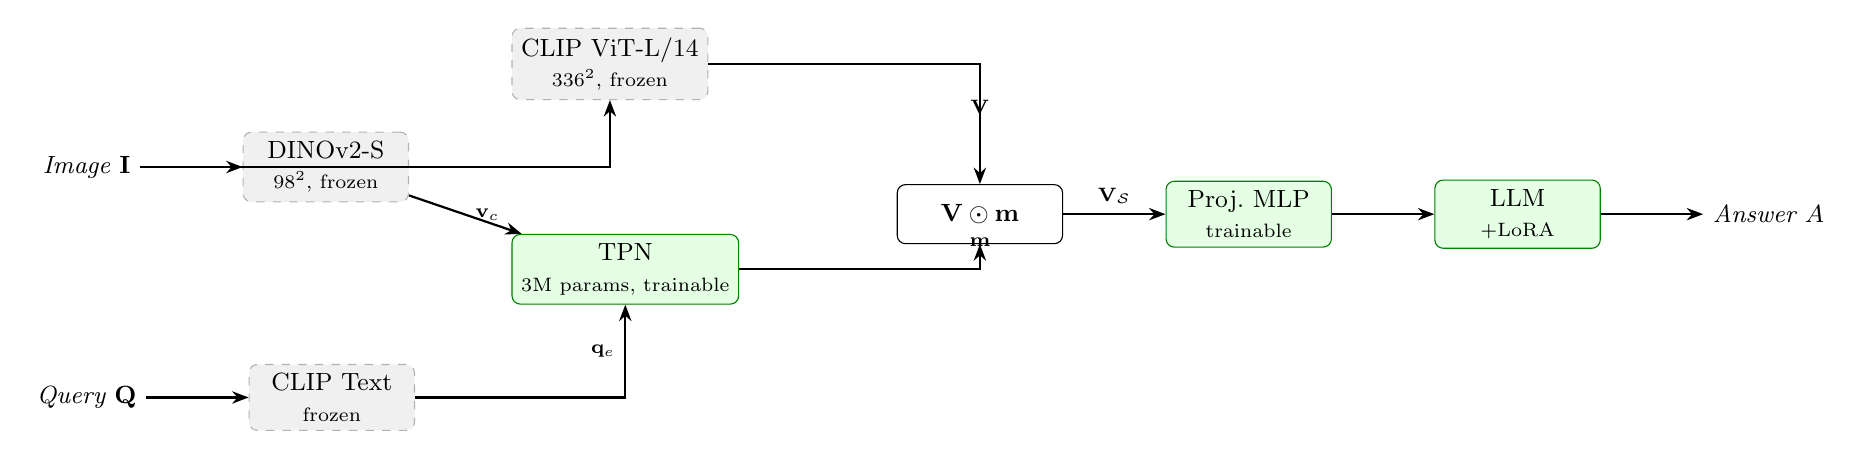
\begin{tikzpicture}[
    node distance=0.7cm and 1.3cm,
    block/.style={rectangle, draw, rounded corners=3pt,
                  minimum height=0.75cm, minimum width=2.1cm,
                  font=\small, align=center, fill=white},
    frozen/.style={block, fill=gray!12, draw=gray!60, dashed},
    trainable/.style={block, fill=green!10, draw=green!50!black},
    data/.style={font=\small\itshape, align=center},
    arr/.style={-{Stealth[scale=0.9]}, thick},
    darr/.style={-{Stealth[scale=0.9]}, thick, dashed, gray}
]
  % Input nodes
  \node[data] (img)   {Image $\mI$};
  \node[data, below=2.4cm of img] (query) {Query $\mQ$};

  % Coarse / text encoders
  \node[frozen, right=of img]   (dino) {DINOv2-S\\{\scriptsize 98$^2$, frozen}};
  \node[frozen, right=of query] (clip) {CLIP Text\\{\scriptsize frozen}};

  % Full ViT (slightly above TPN)
  \node[frozen, above right=0.4cm and 1.3cm of dino] (vit)
    {CLIP ViT-L/14\\{\scriptsize 336$^2$, frozen}};

  % TPN
  \node[trainable, below right=0.4cm and 1.3cm of dino] (tpn)
    {TPN\\{\scriptsize 3M params, trainable}};

  % Mask application
  \node[block, right=2cm of tpn, yshift=0.7cm] (mask) {$\mV \odot \vm$};

  % Projection MLP and LLM
  \node[trainable, right=of mask] (mlp) {Proj.\ MLP\\{\scriptsize trainable}};
  \node[trainable, right=of mlp]  (llm) {LLM\\{\scriptsize +LoRA}};
  \node[data, right=of llm] (ans) {Answer $A$};

  % Arrows
  \draw[arr] (img)   -- (dino);
  \draw[arr] (img)   -| (vit);
  \draw[arr] (query) -- (clip);
  \draw[arr] (dino)  -- (tpn)  node[midway, right, font=\scriptsize] {$\vv_c$};
  \draw[arr] (clip)  -| (tpn)  node[near end, left, font=\scriptsize] {$\vq_e$};
  \draw[arr] (tpn)   -| (mask) node[near end, above, font=\scriptsize] {$\vm$};
  \draw[arr] (vit)   -| (mask) node[near end, above, font=\scriptsize] {$\mV$};
  \draw[arr] (mask)  -- (mlp)  node[midway, above, font=\scriptsize] {$\mV_\mathcal{S}$};
  \draw[arr] (mlp)   -- (llm);
  \draw[arr] (llm)   -- (ans);
\end{tikzpicture}
\caption{TC-ViTok system architecture. Gray dashed boxes are frozen. Green
boxes are trainable. The TPN is the only novel module; it produces a binary
mask conditioned on the query and coarse visual features.}
\label{fig:architecture}
\end{figure}

The TC-ViTok system consists of five components shown in \cref{fig:architecture}:
(1) a coarse visual encoder, (2) a text encoder, (3) the Tokenization Policy
Network (TPN), (4) a full visual encoder with token masking, and (5) the frozen
VLM backbone with LoRA adapters.

\subsection{Coarse Visual Encoder}
\label{subsec:coarse}

\paragraph{Purpose.}
The TPN needs a spatial feature map of the image to decide where to focus.
However, we cannot use the full ViT-L (307M parameters) for this---it would
defeat the efficiency purpose. We instead use DINOv2-Small~\citep{oquab2023dinov2}
at low resolution as a cheap spatial oracle.

\paragraph{Specification.}
\begin{itemize}[leftmargin=2em]
  \item Input: image resized to $98 \times 98$ pixels.
  \item Patch size: 14 pixels $\Rightarrow$ $7 \times 7 = 49$ spatial tokens.
  \item Output: $\vv_c \in \R^{49 \times 384}$ (CLS token excluded).
  \item Parameters: 22M (all frozen during training).
  \item Inference cost: $\approx 3$\,ms on A100.
\end{itemize}

\paragraph{Why DINOv2 and not CLIP-ViT for coarse features?}
DINOv2 is trained with a self-supervised local-feature objective, producing
spatial token representations that correspond faithfully to image regions.
CLIP-ViT is trained to collapse spatial structure into a global embedding for
image-text matching---its intermediate spatial tokens are less geometrically
interpretable and therefore provide weaker spatial guidance to the TPN.

\subsection{Text Encoder}
\label{subsec:text}

\paragraph{Specification.}
\begin{itemize}[leftmargin=2em]
  \item Model: CLIP ViT-B/32 text encoder~\citep{radford2021learning}, all frozen.
  \item Input: tokenized query $\mQ = (q_1, \ldots, q_L)$.
  \item Output: $\vq_e \in \R^{512}$, the [EOS] token embedding.
  \item Why [EOS] and not mean-pooling? CLIP training places the global query
    summary in the [EOS] position. Mean-pooling dilutes this with padding tokens.
\end{itemize}

\begin{intuitionbox}
  \textbf{Why cross-attention can bridge CLIP and DINOv2 spaces.}
  The query embedding ($\vq_e$, CLIP text space, $\R^{512}$) and the coarse
  visual features ($\vv_c$, DINOv2 space, $\R^{384}$) live in \emph{different}
  embedding spaces. The learned projection matrices $\mathbf{W}^Q$ and
  $\mathbf{W}^K$ map both into a shared $d_{\mathrm{model}}$-dimensional space.
  The pre-training of both encoders on semantically meaningful objectives
  provides a favorable initialization landscape for this alignment---but the
  alignment itself must be \emph{learned} by the TPN, not assumed.
\end{intuitionbox}

\subsection{Tokenization Policy Network (TPN)}
\label{subsec:tpn}

The TPN is a lightweight module ($\approx 3$M parameters, all trainable) that
computes spatial relevance scores for each of the $N$ visual tokens, conditioned
on the query.

\subsubsection{Cross-Attention Mechanism}

The TPN's core is a single cross-attention block where the language query attends
to the coarse visual regions.

\begin{mathbox}[title={Cross-Attention in TPN}]
Let $h$ be the number of attention heads and $d_k = d_{\mathrm{model}} / h$.
The query vector $\vq_e \in \R^{d_q}$ (a single vector, not a sequence) is
projected to a single-row query matrix, and the $M$ coarse visual tokens are
projected to keys and values:
\begin{align}
  \mathbf{Q}_{\mathrm{attn}} &= \vq_e^\top \mathbf{W}^Q
    \in \R^{1 \times d_{\mathrm{model}}},
    & \mathbf{W}^Q &\in \R^{d_q \times d_{\mathrm{model}}}
    \label{eq:q_proj} \\
  \mathbf{K}_{\mathrm{attn}} &= \vv_c \mathbf{W}^K
    \in \R^{M \times d_{\mathrm{model}}},
    & \mathbf{W}^K &\in \R^{d_c \times d_{\mathrm{model}}}
    \label{eq:k_proj} \\
  \mathbf{V}_{\mathrm{attn}} &= \vv_c \mathbf{W}^V
    \in \R^{M \times d_{\mathrm{model}}},
    & \mathbf{W}^V &\in \R^{d_c \times d_{\mathrm{model}}}
    \label{eq:v_proj}
\end{align}
For head $h_i$, the attention weights and output are:
\begin{equation}
  \boldsymbol{\alpha}_{h_i} = \Softmax\!\left(
    \frac{\mathbf{Q}_{\mathrm{attn},h_i}\, \mathbf{K}_{\mathrm{attn},h_i}^\top}
      {\sqrt{d_k}}\right) \in \R^{1 \times M}
  \label{eq:attn_weights}
\end{equation}
\begin{equation}
  \mathbf{a}_{h_i} = \boldsymbol{\alpha}_{h_i}\, \mathbf{V}_{\mathrm{attn},h_i}
    \in \R^{1 \times d_k}
  \label{eq:attn_out}
\end{equation}
Multi-head concatenation: $\mathbf{a} = \Concat(\mathbf{a}_{h_1}, \ldots,
\mathbf{a}_{h_H}) \in \R^{1 \times d_{\mathrm{model}}}$.
\end{mathbox}

\paragraph{Interpreting the cross-attention.}
The attention weight $\alpha_{h_i, j}$ in \cref{eq:attn_weights} measures how
much the language query ``matches'' coarse visual region $j$. Because CLIP and
DINOv2 are both trained on semantically meaningful objectives, the learned
projections align their spaces, so a query about ``the red car'' can produce high
$\alpha_{j}$ for image tokens in the region containing the red car. The context
vector $\mathbf{a}$ summarises which visual regions are most relevant.

\begin{remark}
  \textbf{Attention weights as spatial scores.}
  Rather than treating $\mathbf{a}$ as the sole input to the score head,
  we also provide the raw attention weights $\boldsymbol{\alpha} \in \R^M$
  directly to the MLP, preserving the spatial structure:
  \[
    \vs_M = \mathrm{ScoreHead}([\mathbf{a};\, \boldsymbol{\alpha}^\top])
  \]
  where $[;\,]$ denotes concatenation. This residual connection prevents the
  single-vector context $\mathbf{a}$ from becoming an information bottleneck
  for spatial prediction.
\end{remark}

\subsubsection{Spatial Scoring and Upsampling}

\begin{mathbox}[title={Spatial Score Computation}]
The context vector $\mathbf{a} \in \R^{d_{\mathrm{model}}}$ and attention
weights $\boldsymbol{\alpha} \in \R^M$ are concatenated and passed through a
two-layer MLP with GELU activation to produce coarse spatial scores:
\begin{align}
  \mathbf{h} &= \sigma_{\mathrm{GELU}}(\mathbf{W}_1
    [\mathbf{a};\, \boldsymbol{\alpha}^\top] + \mathbf{b}_1) \in \R^{d_h},
    & \mathbf{W}_1 &\in \R^{d_h \times (d_{\mathrm{model}} + M)}
    \label{eq:mlp_hidden} \\
  \vs_M &= \mathbf{W}_2 \mathbf{h} + \mathbf{b}_2 \in \R^M,
    & \mathbf{W}_2 &\in \R^{M \times d_h}
    \label{eq:mlp_output}
\end{align}
These $M = 49$ scores are reshaped to a $7 \times 7$ spatial map and bilinearly
upsampled to the full $\sqrt{N} \times \sqrt{N} = 24 \times 24$ grid:
\begin{equation}
  \vs_N = \flatten\!\left(
    \Upsample\!\left(\reshape(\vs_M, \sqrt{M}, \sqrt{M}),\,
      (\sqrt{N}, \sqrt{N})\right)\right) \in \R^N
  \label{eq:upsample}
\end{equation}
\end{mathbox}

\paragraph{Why bilinear upsampling?}
Spatially relevant regions are typically larger than a single patch---a face
spans many patches, as does a text region. Bilinear upsampling produces spatially
contiguous score patterns, providing a sensible inductive bias: if a coarse
region is relevant, neighbouring fine-grained patches are also likely relevant.

\subsubsection{Token Selection}

At inference time, the top-$k$ tokens by score are selected:
\begin{equation}
  \mathcal{S} = \TopK(\vs_N,\, k) = \{i : s_{N,i}
    \text{ is among the } k \text{ largest values of } \vs_N\}
  \label{eq:topk}
\end{equation}

During training, this discrete operation is replaced by a differentiable
approximation (see \cref{sec:gumbel}).

\subsection{Full Visual Encoder and Token Masking}

\paragraph{CLIP ViT-L/14 (frozen).}
The primary visual encoder produces embeddings $\mV \in \R^{576 \times 1024}$
from the full $336 \times 336$ image. We do not modify it.

\paragraph{Mask application.}
Given the binary mask $\vm \in \{0,1\}^N$ from the TPN, the masked visual
tokens are defined element-wise as:
\begin{equation}
  (\mV_\mathcal{S})_i = m_i \cdot \mathbf{V}_i, \quad i = 1, \ldots, N
  \label{eq:masking}
\end{equation}
where $\mathbf{V}_i \in \R^{d_v}$ is the $i$-th row of $\mV$. Unselected tokens
become zero vectors. Positional embeddings of selected tokens are preserved,
maintaining spatial coherence for the downstream LLM.

\begin{remark}
  \label{rem:pre_vit}
  \textbf{On pre-ViT vs.\ post-ViT savings.} In the current implementation,
  the full ViT-L processes all $N$ tokens before masking. Computational savings
  are realized only in the LLM (shorter effective context when using
  \texttt{torch.gather} to extract $k$ tokens). True pre-ViT savings---where
  unselected patches skip ViT self-attention---would require a sparse-attention
  ViT, which we leave to future work. Nevertheless, LLM-side savings are
  substantial: reducing visual tokens from 576 to 144 cuts prefill cost by
  $\approx 70\%$ for the dominant $O(N \cdot (N+L))$ term.
\end{remark}

\begin{implbox}
  Two implementation strategies for \cref{eq:masking}:
  \begin{enumerate}[leftmargin=1.5em]
    \item \textbf{Zero masking}: Multiply full sequence by $\vm$, keeping
      length $N$. Simple; no padding complexity. Saves only LLM context memory,
      not compute.
    \item \textbf{Gather}: Use \texttt{torch.gather} to extract only selected
      tokens, producing a sequence of length $k$. Saves both LLM compute and
      memory. Requires variable-length batch handling. Recommended for the
      published efficiency numbers.
  \end{enumerate}
  For course project implementation, use Option~1. For the final paper's
  latency measurements, use Option~2.
\end{implbox}

\subsection{Projection MLP and LLM Backbone}

The masked visual tokens pass through LLaVA-1.5's two-layer MLP projector,
mapping $\R^{d_v} \to \R^{d_{\mathrm{LLM}}}$ (e.g., $1024 \to 4096$ for
Vicuna-7B). This projector is trainable in Phase~1. The projected tokens are
concatenated with text token embeddings and processed by the LLM backbone, with
LoRA adapters applied to the attention projection matrices $\{Q, K, V, O\}$.

% ════════════════════════════════════════════════════════════════════════════
\section{Differentiable Token Selection}
\label{sec:gumbel}
% ════════════════════════════════════════════════════════════════════════════

\subsection{The Non-Differentiability Problem}

The core training challenge is that $\TopK(\vs_N, k)$ is a discrete operation
with zero gradients almost everywhere. For $\vm = \mathbf{1}[\vs_N \geq
\tau_k(\vs_N)]$ where $\tau_k$ is the $k$-th largest value:
\[
  \frac{\partial \vm}{\partial \vs_N} = \mathbf{0}
    \quad \text{(almost everywhere)}
\]
This means gradients cannot flow from the VQA loss through the mask to the TPN
parameters $\theta$. We need a differentiable approximation.

\subsection{Gumbel-Sigmoid for Per-Token Selection}

For binary per-token selection (as opposed to categorical one-of-$N$ selection),
we use the Gumbel-Sigmoid rather than the Gumbel-Softmax. This is a critical
distinction: Gumbel-Softmax produces a distribution over $N$ options summing to
1 (i.e., ``choose one token''), which is inappropriate for top-$k$ selection.
Gumbel-Sigmoid treats each token independently.

\begin{mathbox}[title={Gumbel-Sigmoid for Independent Binary Selection}]
Let $\mathbf{g} \in \R^N$ be i.i.d.\ Gumbel noise:
$g_i = -\log(-\log(u_i + \epsilon) + \epsilon)$,  $u_i \sim \mathrm{Uniform}(0,1)$,
with $\epsilon = 10^{-8}$ for numerical stability. The Gumbel-Sigmoid soft mask is:
\begin{equation}
  \tilde{m}_i(\tau) = \sigma\!\left(\frac{s_{N,i} + g_i}{\tau}\right)
    = \frac{1}{1 + \exp\!\left(-\frac{s_{N,i} + g_i}{\tau}\right)}
  \label{eq:gumbel_sigmoid}
\end{equation}
Each $\tilde{m}_i \in (0,1)$ is an independent soft selection probability.
As $\tau \to 0$, $\tilde{m}_i \to \mathbf{1}[s_{N,i} + g_i > 0]$ (nearly binary).
As $\tau \to \infty$, $\tilde{m}_i \to 0.5$ (near-uniform).
\end{mathbox}

\subsection{Straight-Through Estimator}

\begin{mathbox}[title={Straight-Through Estimator (STE)}]
The STE uses the hard top-$k$ mask in the forward pass but the soft
Gumbel-Sigmoid for gradient computation in the backward pass:
\begin{align}
  \vm_{\mathrm{hard}} &= \mathbf{1}[\vs_N \geq \tau_k(\vs_N)]
    && \text{(hard top-}k\text{ mask, forward)} \label{eq:hard} \\
  \tilde{\vm}(\tau) &= \sigma((\vs_N + \mathbf{g}) / \tau)
    && \text{(Gumbel-Sigmoid, backward)} \label{eq:soft} \\
  \vm_{\mathrm{STE}} &= \vm_{\mathrm{hard}}
    - \tilde{\vm}(\tau).\mathrm{stop\_grad}() + \tilde{\vm}(\tau)
    \label{eq:ste}
\end{align}
Forward pass: $\vm_{\mathrm{STE}} = \vm_{\mathrm{hard}}$ (exact integer mask).
Backward pass: $\partial \vm_{\mathrm{STE}} / \partial \vs_N =
\partial \tilde{\vm} / \partial \vs_N$ (smooth Gumbel-Sigmoid gradient).
\end{mathbox}

\paragraph{PyTorch implementation.}

\begin{lstlisting}[caption={Gumbel-Sigmoid STE for top-$k$ selection.}]
import torch
import torch.nn.functional as F

def gumbel_sigmoid_ste(scores, k, tau):
    """
    scores: (B, N) raw spatial scores from TPN
    k:      int, number of tokens to select
    tau:    float, Gumbel temperature (annealed during training)
    Returns: mask (B, N) with STE for gradients
    """
    # Gumbel-Sigmoid soft mask
    eps = 1e-8
    noise = -torch.log(-torch.log(
        torch.rand_like(scores).clamp(eps, 1 - eps)) + eps)
    m_soft = torch.sigmoid((scores + noise) / tau)

    # Hard top-k mask (forward pass)
    topk_idx = scores.topk(k, dim=-1).indices
    m_hard = torch.zeros_like(scores).scatter_(-1, topk_idx, 1.0)

    # STE: forward uses m_hard, backward uses m_soft
    # m_hard - m_soft.detach() + m_soft evaluates to m_hard in fwd
    # but carries grad through m_soft in bwd
    return m_hard - m_soft.detach() + m_soft
\end{lstlisting}

\paragraph{Gradient bias of STE.}
The STE introduces bias because $\partial \vm_{\mathrm{hard}} / \partial \vs \neq
\partial \tilde{\vm} / \partial \vs$. However, as shown by~\citet{bengio2013estimating},
bias is acceptable when variance is low, and STE achieves this by using the full
sigmoid gradient rather than a high-variance Monte Carlo estimate (REINFORCE).
For binary masks of dimension $N = 576$, REINFORCE variance is prohibitively high.

\paragraph{Temperature annealing.}
We anneal $\tau$ from $\tau_{\max} = 1.0$ (very soft, high-quality gradients,
slow convergence) to $\tau_{\min} = 0.1$ (nearly hard, noisy gradients, fast
convergence):
\begin{equation}
  \tau(t) = \tau_{\min} + (\tau_{\max} - \tau_{\min})
    \cdot \left(1 - \frac{t}{T}\right)
  \label{eq:tau_anneal}
\end{equation}
where $t$ is the current step and $T$ is total training steps.

\begin{intuitionbox}
  \textbf{Why anneal?} At high $\tau$, the Gumbel-Sigmoid mask $\tilde{\vm}$ is
  nearly uniform ($\approx 0.5$ everywhere). This means the gradient
  $\partial \tilde{m}_i / \partial s_i = \tilde{m}_i(1 - \tilde{m}_i) \approx
  0.25$ is large for \emph{every} token---a rich, low-variance learning signal.
  As $\tau$ decreases, the gradient concentrates on the selected tokens. Late
  training thus resembles learning from hard decisions, which is the correct
  inference-time behavior.
\end{intuitionbox}

% ════════════════════════════════════════════════════════════════════════════
\section{Training Dynamics}
\label{sec:training}
% ════════════════════════════════════════════════════════════════════════════

\subsection{Gradient Flow Path}

\begin{figure}[t]
\centering
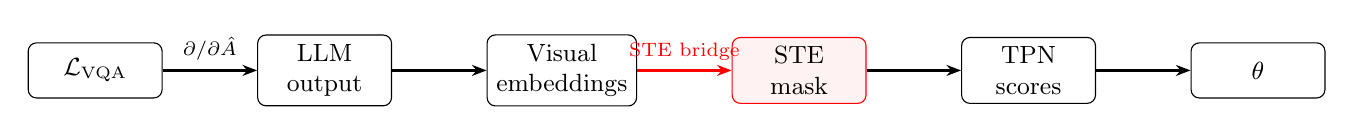
\begin{tikzpicture}[
    node distance=0.4cm and 1.2cm,
    block/.style={rectangle, draw, rounded corners=3pt,
                  minimum height=0.7cm, minimum width=1.7cm,
                  font=\small, align=center, fill=white},
    arr/.style={-{Stealth[scale=0.8]}, thick},
    rarr/.style={-{Stealth[scale=0.8]}, thick, red}
]
  \node[block] (loss)   {$\mathcal{L}_{\mathrm{VQA}}$};
  \node[block, right=of loss] (llm)    {LLM\\output};
  \node[block, right=of llm]  (emb)    {Visual\\embeddings};
  \node[block, right=of emb,
        draw=red, fill=red!5]  (ste)    {STE\\mask};
  \node[block, right=of ste]  (scores) {TPN\\scores};
  \node[block, right=of scores](theta) {$\theta$};

  \draw[arr]  (loss)   -- (llm)
    node[midway, above, font=\scriptsize]{$\partial/\partial\hat{A}$};
  \draw[arr]  (llm)    -- (emb);
  \draw[rarr] (emb)    -- (ste)
    node[midway, above, font=\scriptsize, red]{STE bridge};
  \draw[arr]  (ste)    -- (scores);
  \draw[arr]  (scores) -- (theta);
\end{tikzpicture}
\caption{Gradient flow from VQA loss to TPN parameters. The STE (red) is
the critical differentiable bridge across the discrete mask.}
\label{fig:grad_flow}
\end{figure}

The gradient from the VQA loss flows through the chain shown in
\cref{fig:grad_flow}. Without the STE, all gradient mass above the mask is
zeroed out and $\theta$ receives no useful learning signal.

\subsection{Full Training Loss}

The total training loss at step $t$ is:
\begin{equation}
  \mathcal{L}(t) = \mathcal{L}_{\mathrm{VQA}}
    + \lambda(t) \cdot \frac{\|\vs_N\|_1}{N}
  \label{eq:total_loss}
\end{equation}
Minimizing $\|\vs_N\|_1$ encourages most scores to be near zero, which via the
Gumbel-Sigmoid drives the soft mask to be sparse.

\paragraph{Lambda annealing schedule.}
\begin{equation}
  \lambda(t) = \lambda_{\max} \cdot
    \min\!\left(1,\; \frac{t}{T_{\mathrm{warmup}}}\right)
  \label{eq:lambda_anneal}
\end{equation}
Starting with $\lambda = 0$ lets the TPN learn which tokens are useful
(accuracy-focused) before being penalized for using too many.

\subsection{Phased Training Protocol}

\paragraph{Phase 0: TPN warm-up (1 epoch, TPN only).}
Only TPN parameters are trained. LLM, ViT-L, DINOv2-S, CLIP text, and projection
MLP are all frozen. Loss: $\mathcal{L}_{\mathrm{VQA}}$ only ($\lambda = 0$).
Temperature $\tau = 1.0$.

\textbf{Why Phase~0 is essential: the cold-start problem.} Without warm-up, the
TPN starts with random weights and produces near-random masks. A large frozen
LLM can often answer VQA questions using language priors alone, meaning the VQA
gradient flowing to the TPN is very weak in early Phase~1 training---the LLM
routes around the visual channel. Phase~0 forces the TPN to learn in isolation:
with only TPN parameters changing, the only way to improve VQA accuracy is to
select better tokens.

\paragraph{Phase 1: Joint fine-tuning (3 epochs, TPN + LoRA + MLP).}
Trainable: TPN, LoRA adapters (rank 32), projection MLP. Frozen: ViT-L,
DINOv2-S, CLIP text, LLM body. Loss: $\mathcal{L}(t)$ with $\lambda$ and $\tau$
annealing per \cref{eq:lambda_anneal,eq:tau_anneal}.

\paragraph{Phase 2: Domain transfer (optional, 1 epoch, fine-grained tasks).}
Fine-tune on target domain (GQA, TextVQA) with $\lambda = 0$, $\tau = 0.1$
(near-hard). Tests whether the learned policy generalizes to unseen distributions.

\begin{algorithm}[t]
\caption{TC-ViTok Training}
\label{alg:training}
\begin{algorithmic}[1]
\Require Dataset $\mathcal{D}$, token budget $k$, $\lambda_{\max}$, steps $T$
\State Initialize TPN $\theta$ randomly; load pretrained frozen encoders
\State Apply LoRA (rank=32, $\alpha$=64) to LLM $\{Q,K,V,O\}$ projections
\Statex \textbf{--- Phase 0: TPN warm-up ---}
\For{$e = 1, \ldots, E_0$}
  \For{$(\mI, \mQ, A)$ in $\mathcal{D}$}
    \State $\vv_c \leftarrow \mathrm{DINOv2\text{-}S}(\mathrm{resize}(\mI, 98^2))$
    \State $\vq_e \leftarrow \mathrm{CLIPText}(\mQ)$
    \State $\vs_N \leftarrow \mathrm{TPN}_\theta(\vv_c, \vq_e)$
    \State $\vm \leftarrow \mathrm{STE}(\vs_N, k, \tau{=}1.0)$
    \State $\mV \leftarrow \mathrm{ViT\text{-}L}(\mI)$
    \State $\hat{A} \leftarrow f_{\mathrm{LLM}}(\mQ,\, \mV \odot \vm)$ \Comment{LLM frozen}
    \State $\mathcal{L} \leftarrow \mathcal{L}_{\mathrm{VQA}}(\hat{A}, A)$
    \State $\theta \leftarrow \theta - \eta_{\mathrm{TPN}} \nabla_\theta \mathcal{L}$
  \EndFor
\EndFor
\Statex \textbf{--- Phase 1: Joint fine-tuning ---}
\For{$t = 1, \ldots, T$}
  \State Sample $(\mI, \mQ, A) \sim \mathcal{D}$
  \State $\tau \leftarrow \tau(t)$ via \cref{eq:tau_anneal};
         $\quad \lambda \leftarrow \lambda(t)$ via \cref{eq:lambda_anneal}
  \State Compute $\vs_N$, $\vm$ as above
  \State $\hat{A} \leftarrow f_{\mathrm{LLM}}^{\mathrm{LoRA}}(\mQ,\, \mV \odot \vm)$
  \State $\mathcal{L} \leftarrow \mathcal{L}_{\mathrm{VQA}}(\hat{A}, A)
    + \lambda\,\|\vs_N\|_1 / N$
  \State Update $\theta$, LoRA, MLP via AdamW; clip $\|\nabla_\theta\|_2 \leq 1$
\EndFor
\end{algorithmic}
\end{algorithm}

% ════════════════════════════════════════════════════════════════════════════
\section{Failure Modes and Mitigations}
\label{sec:failures}
% ════════════════════════════════════════════════════════════════════════════

\subsection{Spatial Collapse (Center Bias)}

\begin{warnbox}[title={Failure Mode 1: Spatial Collapse}]
\textbf{Symptom:} The TPN consistently selects center-image tokens regardless of
the query. On a $24 \times 24$ selection heatmap, selected tokens form a
circular blob at the image center.

\textbf{Cause:} Natural images are heavily center-biased (photographers place
subjects at center). The TPN learns this statistical prior rather than the
task-specific signal.

\textbf{Diagnosis:} Compute the mean selected-token centroid across 1000
validation examples:
\[
  \bar{\mathbf{c}} = \frac{1}{|\mathcal{D}_{\mathrm{val}}|}
    \sum_{(\mI,\mQ)} \frac{\sum_{i \in \mathcal{S}} \mathbf{p}_i}{k}
\]
where $\mathbf{p}_i \in \R^2$ is the $(x,y)$ coordinate of token $i$. If
$\|\bar{\mathbf{c}} - \mathbf{c}_{\mathrm{center}}\|_2 < \epsilon$, collapse
has occurred.
\end{warnbox}

\paragraph{Fix: Spatial entropy regularizer.}
We encourage the TPN to use diverse spatial positions by maximizing the entropy
of the mean selection distribution across a batch. Define the normalized batch
selection frequency:
\[
  \hat{p}_i = \frac{\bar{m}_i}{\sum_{j=1}^N \bar{m}_j + \epsilon},
  \quad \bar{m}_i = \frac{1}{B} \sum_{b=1}^B m_i^{(b)}
\]
where $\epsilon = 10^{-8}$ ensures numerical stability and $\hat{p}$ sums to 1.
Then maximize the Shannon entropy:
\begin{equation}
  \mathcal{L}_{\mathrm{entropy}} = -\sum_{i=1}^N
    \hat{p}_i \log(\hat{p}_i + \epsilon)
  \label{eq:entropy_reg}
\end{equation}
This is \emph{subtracted} from the total loss (i.e., we maximize entropy) with a
small coefficient $\mu = 0.01$.

\subsection{Query Ignoring}

\begin{warnbox}[title={Failure Mode 2: Query Ignoring}]
\textbf{Symptom:} The selected token sets for the same image with two different
queries are nearly identical.
Quantitatively: $\IoU(\mathcal{S}(\mQ_1, \mI), \mathcal{S}(\mQ_2, \mI)) \approx 1$.

\textbf{Cause:} The TPN ignores $\vq_e$ and makes decisions based on image content
alone. This happens when: (1) Phase~0 training is too short and the query pathway
is not established; (2) the projection $\mathbf{W}^Q$ collapses to near-zero.

\textbf{Diagnosis:} For the same image, compute selected token sets for 10 diverse
queries. Compute pairwise IoU. If mean IoU $> 0.9$, query ignoring is occurring.
\end{warnbox}

\paragraph{Fix: Query-diversity contrastive loss.}
For each batch, sample pairs of queries $(\mQ_1^{(b)}, \mQ_2^{(b)})$ per image.
Penalize mask similarity when the queries are semantically different:
\begin{equation}
  \mathcal{L}_{\mathrm{div}} = \sum_{b=1}^B \max\!\left(
    0,\; \simop(\vm_1^{(b)},\, \vm_2^{(b)}) - \gamma
  \right) \cdot \left(1 - \simop(\vq_{e,1}^{(b)},\, \vq_{e,2}^{(b)})\right)
  \label{eq:div_loss}
\end{equation}
where $\simop(\mathbf{a}, \mathbf{b}) = \mathbf{a}^\top \mathbf{b} /
(\|\mathbf{a}\|\|\mathbf{b}\|)$ is cosine similarity. The factor
$(1 - \simop(\vq_{e,1}, \vq_{e,2}))$ ensures no penalty when queries are similar.

\subsection{Degenerate Fixed Masks}

\begin{warnbox}[title={Failure Mode 3: Degenerate Fixed Mask}]
\textbf{Symptom:} The TPN selects the exact same $k$ tokens for every image and
every query. Both spatial diversity and query sensitivity are zero.

\textbf{Cause:} $\lambda$ was increased too aggressively, forcing the TPN to
find the single ``safest'' $k$ tokens (those informative on average across the
training distribution). The compression loss dominates the VQA loss.

\textbf{Fix:} Reset $\lambda = 0$, reduce $\lambda_{\max}$ by $10\times$,
increase $T_{\mathrm{warmup}}$. Also reduce the LoRA learning rate---a
too-quickly-adapting LLM can make the TPN unnecessary by memorizing fixed
token patterns.
\end{warnbox}

\paragraph{Additional note: train-test mask discrepancy.}
During training, the Gumbel-Sigmoid produces soft masks in $(0,1)^N$ whose sum
is not exactly $k$. At inference, the hard top-$k$ mask has exactly $k$ ones.
This train-test discrepancy is an inherent limitation of the STE approach.
In practice, the gap is small because temperature annealing drives the soft masks
near-binary by late training.

% ════════════════════════════════════════════════════════════════════════════
\section{Implementation Plan}
\label{sec:implementation}
% ════════════════════════════════════════════════════════════════════════════

\subsection{Phase A: Baseline Reproduction}

\textbf{Goal:} Run LLaVA-1.5 on VQAv2 and confirm 79.1\% accuracy.

\textbf{Key steps:}
\begin{enumerate}[leftmargin=2em]
  \item Install: \texttt{transformers$\geq$4.36}, \texttt{accelerate},
    \texttt{datasets}, \texttt{pillow}, \texttt{peft}.
  \item Load \texttt{llava-hf/llava-1.5-7b-hf} (use 1.5, not 1.6; 1.6 uses
    dynamic tiling that complicates token-level surgery).
  \item Use the official VQA evaluation script for accuracy---not a custom
    function. Answer normalization is subtle and will give wrong numbers otherwise.
  \item Record baseline inference time with \texttt{torch.cuda.Event} and
    \texttt{synchronize()}. This is the denominator for your speedup claims.
\end{enumerate}

\textbf{First paper figure:} Run PCA on the 576 visual tokens and visualize the
first 3 components as RGB in the $24 \times 24$ spatial grid. This should show
smooth spatial structure, confirming tokens are spatially organized and the TPN
can meaningfully score them.

\subsection{Phase B: Token Extraction and Caching}

\begin{lstlisting}[caption={Forward hook to intercept ViT-L output tokens.}]
# Hook into the last ViT-L encoder layer
visual_tokens_cache = []

def hook_fn(module, input, output):
    visual_tokens_cache.append(output.detach().cpu())

# Path is specific to HuggingFace llava-hf; verify for other implementations
hook = model.model.vision_tower \
    .vision_model.encoder.layers[-1] \
    .register_forward_hook(hook_fn)

with torch.no_grad():
    output = model(**inputs)

hook.remove()
print(visual_tokens_cache[0].shape)  # Expected: (1, 576, 1024)
\end{lstlisting}

\begin{implbox}
  \textbf{Caching strategy.} Pre-compute and cache all coarse ViT features and
  CLIP text embeddings to HDF5 before training:
  \begin{lstlisting}[numbers=none]
import h5py
with h5py.File('cached_features.h5', 'w') as f:
    f.create_dataset('coarse', shape=(N, 49, 384), dtype='float16')
    f.create_dataset('query',  shape=(N, 512),     dtype='float16')
  \end{lstlisting}
  For 100K samples, this is $\approx$4\,GB and saves hours of compute per epoch.
  Different normalizations apply: CLIP uses its own mean/std; DINOv2 uses ImageNet
  statistics. Using the wrong normalization is a silent, hard-to-debug error.
\end{implbox}

\subsection{Phase C: TPN Implementation}

Implement the \texttt{TokenizationPolicyNetwork} class with:
\begin{itemize}[leftmargin=2em]
  \item \texttt{d\_img = 384} (DINOv2-S output dimension)
  \item \texttt{d\_query = 512} (CLIP-B/32 text output dimension)
  \item \texttt{d\_model = 256} (shared projection dimension)
  \item \texttt{d\_h = 256} (hidden MLP dimension)
  \item \texttt{n\_heads = 2}
  \item \texttt{n\_spatial = 49}; \texttt{n\_full = 576}
\end{itemize}

\begin{lstlisting}[caption={Core TPN forward pass.}]
class TPN(nn.Module):
    def forward(self, v_coarse, q_embed, k, tau, training=True):
        # Project to shared space
        Q = self.q_proj(q_embed).unsqueeze(1)   # (B, 1, d_model)
        K = self.img_proj(v_coarse)              # (B, 49, d_model)
        V = K  # shared key/value projection

        # Cross-attention
        ctx, alpha = self.cross_attn(Q, K, V)   # ctx: (B,1,d_model)
        alpha = alpha.squeeze(1)                 # (B, 49)

        # Score head with attention residual
        combined = torch.cat([ctx.squeeze(1), alpha], dim=-1)
        coarse_scores = self.score_head(combined)  # (B, 49)

        # Upsample to (B, 576)
        s = coarse_scores.view(-1, 1, 7, 7)
        s = F.interpolate(s, (24, 24), mode='bilinear', align_corners=False)
        s = s.view(-1, 576)

        if training:
            mask = gumbel_sigmoid_ste(s, k, tau)
        else:
            topk_idx = s.topk(k, dim=-1).indices
            mask = torch.zeros_like(s).scatter_(-1, topk_idx, 1.0)
        return mask, s
\end{lstlisting}

\textbf{Critical debugging check:} After a forward+backward pass, verify that
\texttt{mask.grad\_fn is not None}. If it is \texttt{None}, the STE is broken
and $\theta$ receives no gradient.

\subsection{Phase D: Integration into LLaVA}

Wrap LLaVA in a \texttt{TCViTok} module. The visual token flow:
\begin{enumerate}[leftmargin=2em]
  \item $\mI \to$ ViT-L $\to$ $\mV \in \R^{576 \times 1024}$ (frozen)
  \item $\mI_c \to$ DINOv2-S $\to$ $\vv_c \in \R^{49 \times 384}$ (frozen)
  \item $\mQ \to$ CLIP-text $\to$ $\vq_e \in \R^{512}$ (frozen)
  \item $(\vv_c, \vq_e) \to$ TPN $\to$ $\vm \in \{0,1\}^{576}$ (trainable)
  \item $\mV \odot \vm \to$ MLP projector $\to$ $\R^{576 \times 4096}$ (trainable)
  \item Concat with text embeddings $\to$ LLM $\to$ answer
\end{enumerate}

\begin{lstlisting}[caption={LoRA setup via PEFT library.}]
from peft import get_peft_model, LoraConfig, TaskType

lora_config = LoraConfig(
    task_type=TaskType.CAUSAL_LM,
    r=32,             # rank
    lora_alpha=64,
    target_modules=["q_proj","k_proj","v_proj","o_proj"],
    lora_dropout=0.05,
    bias="none"
)
model.llava = get_peft_model(model.llava, lora_config)
model.llava.print_trainable_parameters()
# Expected: ~1-2% of total parameters are trainable
\end{lstlisting}

\subsection{Phase E: Training Loop}

\begin{lstlisting}[caption={Core training step.}]
def train_step(batch, model, optimizer, step, T, T_warmup, lam_max):
    pixel_values = batch['pixel_values'].to(device)
    input_ids    = batch['input_ids'].to(device)
    labels       = batch['labels'].to(device)

    tau = get_tau(step, T)          # Equation 13
    lam = get_lambda(step, T_warmup, lam_max)  # Equation 14

    outputs, s_N = model(pixel_values, input_ids, labels, tau)
    L_vqa  = outputs.loss
    L_comp = s_N.abs().mean()       # L1 sparsity proxy

    loss = L_vqa + lam * L_comp
    loss.backward()

    torch.nn.utils.clip_grad_norm_(model.tpn.parameters(), 1.0)
    optimizer.step()
    optimizer.zero_grad()
    return L_vqa.item(), L_comp.item()
\end{lstlisting}

\textbf{Optimizer:} AdamW with $\eta_{\mathrm{TPN}} = 10^{-3}$,
$\eta_{\mathrm{LoRA}} = 2 \times 10^{-4}$, $\eta_{\mathrm{MLP}} = 5 \times
10^{-4}$, weight decay $= 0.01$.
Per-GPU batch size 1 with 8 gradient accumulation steps (effective batch size 8).
Enable gradient checkpointing: \texttt{model.gradient\_checkpointing\_enable()}.

\subsection{Phase F: Evaluation}

\begin{enumerate}[leftmargin=2em]
  \item Run at $k \in \{72, 144, 216, 288, 576\}$ to generate Pareto curve.
  \item For each $k$: report VQAv2-val, GQA-balanced, POPE-adversarial.
  \item Stratify by spatial/global question type (see \cref{sec:experiments}).
  \item Compute mean selected-token centroid and IoU across query pairs to
    check for spatial collapse and query ignoring.
\end{enumerate}

% ════════════════════════════════════════════════════════════════════════════
\section{Experimental Design}
\label{sec:experiments}
% ════════════════════════════════════════════════════════════════════════════

\subsection{Baselines}

All conditions use the same LLaVA-1.5-7B (or 3B for lean experiments) backbone
at $k = 144$ tokens ($4\times$ compression from 576):

\begin{center}
\renewcommand{\arraystretch}{1.2}
\begin{tabular}{@{}lllll@{}}
  \toprule
  Baseline & Query-aware & Stage & Tokens & Notes \\
  \midrule
  LLaVA-1.5 (full)    & N/A & None     & 576 & Upper bound \\
  Random drop         & No  & Pre-LLM  & 144 & Lower bound \\
  ToMe (approx.)      & No  & In ViT   & 144 & Content-adaptive \\
  Image-only TPN (A3) & No  & Pre-LLM  & 144 & Ablation: no query \\
  \textbf{TC-ViTok (ours)} & \textbf{Yes} & \textbf{Pre-LLM}
    & \textbf{144} & \textbf{Full method} \\
  \bottomrule
\end{tabular}
\end{center}

\paragraph{Approximating ToMe without the full codebase.}
We approximate ToMe's bipartite soft matching with $k$-means clustering of the
576 ViT-L tokens (k=144), taking the centroid-nearest token per cluster. This
captures ToMe's core mechanism (merge similar tokens) without the $r$-scheduling.
\emph{Caveat:} this approximation may understate ToMe's actual performance;
we also run the official \texttt{tome} package as a sanity check.

\subsection{Datasets}

\begin{itemize}[leftmargin=2em]
  \item \textbf{VQAv2}~\citep{goyal2017vqa}: 214K images, 1.1M QA pairs.
    Primary evaluation benchmark. Lean experiments: 100K stratified subset.
  \item \textbf{GQA}~\citep{hudson2019gqa}: 22M compositionally generated QA
    pairs. Used for spatial question analysis (annotation includes spatial
    relation metadata).
  \item \textbf{TextVQA}: OCR-dependent VQA; tests fine-grained spatial
    allocation to text regions.
  \item \textbf{POPE}~\citep{pope}: adversarial binary question set for
    hallucination evaluation.
\end{itemize}

\subsection{Metrics}

\begin{itemize}[leftmargin=2em]
  \item \textbf{VQA-Score}: official VQAv2 accuracy.
  \item \textbf{GQA accuracy}: exact-match on balanced GQA test set.
  \item \textbf{POPE F1}: F1 score on adversarial POPE set.
  \item \textbf{Latency reduction}: end-to-end inference time vs.\ full
    LLaVA-1.5 at batch size 1 on A100.
\end{itemize}

\subsection{Spatial Specificity Evaluation Protocol}

A question is classified as \emph{spatially specific} by the following priority:
\begin{enumerate}[leftmargin=2em]
  \item (GQA only) Semantic annotation includes \texttt{relation.spatial = True}.
  \item Answer is a spatial direction: \{``left,'' ``right,'' ``top,'' ``bottom''\}.
  \item Question contains spatial relational words:
    \{``left,'' ``right,'' ``above,'' ``below,'' ``next to,'' ``behind,''
    ``corner,'' ``between,'' ``near''\}.
\end{enumerate}
GQA's semantic annotations (criterion 1) are the most reliable source; keyword
matching (criterion 3) is a fallback for VQAv2, which lacks such annotations.
Our primary hypotheses are:
\begin{align}
  &\text{Acc}(A1,\, \mathrm{spatial}) > \text{Acc}(A3,\, \mathrm{spatial})
    \label{eq:hyp1} \\
  &|\text{Acc}(A1,\, \mathrm{global}) - \text{Acc}(A3,\, \mathrm{global})|
    \approx 0 \label{eq:hyp2}
\end{align}
i.e., query-conditioning helps on spatial questions and is neutral on global ones.

\subsection{Ablation Studies}

\paragraph{Must-do ablations (A1--A6):}

\begin{center}
\renewcommand{\arraystretch}{1.2}
\begin{tabular}{@{}lll@{}}
  \toprule
  Ablation & Component removed & Conclusion enabled \\
  \midrule
  A1: Full TC-ViTok   & ---           & Full system performance \\
  A2: Random drop     & TPN entirely  & Absolute lower bound \\
  A3: Image-only TPN  & Query encoder & Value of query conditioning \\
  A4: ToMe (approx.)  & TPN           & SOTA comparison \\
  A5: $k$ sweep       & ---           & Pareto frontier \\
  A6: Question-type split & ---       & Spatial hypothesis validation \\
  \bottomrule
\end{tabular}
\end{center}

\paragraph{Optional ablations (B1--B4):}

\begin{center}
\renewcommand{\arraystretch}{1.2}
\begin{tabular}{@{}lll@{}}
  \toprule
  Ablation & Variation & Tests \\
  \midrule
  B1: TPN depth   & 1 vs.\ 3 cross-attn layers  & Capacity requirements \\
  B2: Coarse enc. & DINOv2-S vs.\ CLIP-ViT-B    & Encoder suitability \\
  B3: No Phase~0  & Skip TPN warm-up            & Cold-start importance \\
  B4: Fixed $\tau$ & $\tau{=}1.0$ throughout    & Annealing importance \\
  \bottomrule
\end{tabular}
\end{center}

% ════════════════════════════════════════════════════════════════════════════
\section{Expected Results and Hypotheses}
\label{sec:results}
% ════════════════════════════════════════════════════════════════════════════

\subsection{Primary Hypotheses}

\begin{proposition}[Query-Conditioning Hypothesis]
  For spatially-grounded VQA questions, TC-ViTok (A1) achieves strictly higher
  accuracy than image-only TPN (A3) at the same token budget $k$. For
  globally-answerable questions, A1 and A3 perform comparably.
  \label{prop:main}
\end{proposition}

\begin{proposition}[Pareto Dominance Hypothesis]
  The accuracy-vs-tokens Pareto curve of TC-ViTok lies at or above the Pareto
  curves of ToMe and random drop for all $k \in \{72, 144, 216, 288\}$.
  \label{prop:pareto}
\end{proposition}

\subsection{Projected Quantitative Outcomes}

\begin{table}[h]
\centering
\caption{Projected results (not measured). Numbers are estimates based on method
structure and prior literature. \emph{All values will be replaced by measured
results in the final submission.}}
\label{tab:projected}
\renewcommand{\arraystretch}{1.2}
\begin{tabular}{@{}lccccc@{}}
  \toprule
  Method & VQAv2 & GQA & GQA-spatial & POPE-F1 & Tokens \\
  \midrule
  LLaVA-1.5 (full)    & 79.1 & 63.3 & 62.1 & 85.9 & 576 \\
  Random drop         & $\sim$72 & $\sim$57 & $\sim$53 & $\sim$81 & 144 \\
  ToMe (approx.)      & $\sim$74 & $\sim$59 & $\sim$55 & $\sim$83 & 144 \\
  Image-only TPN (A3) & $\sim$75 & $\sim$60 & $\sim$56 & $\sim$83 & 144 \\
  \textbf{TC-ViTok (ours)} & $\mathbf{\sim76}$ & $\mathbf{\sim61}$
    & $\mathbf{\sim59}$ & $\mathbf{\sim84}$ & 144 \\
  \bottomrule
\end{tabular}
\end{table}

The key predicted pattern: TC-ViTok's advantage over A3 is concentrated in
GQA-spatial ($+3$ projected points) rather than overall VQA ($+1$ projected
point), validating \cref{prop:main}.

\subsection{Interpreting Weaker-Than-Expected Results}

If overall VQA improvement is $< 0.5$ points, the paper remains valid if:
\begin{itemize}[leftmargin=2em]
  \item The spatial/global split shows the predicted asymmetry
    (\cref{eq:hyp1,eq:hyp2}).
  \item The Pareto curve shows query-conditioning's advantage grows with
    compression ratio---at $k = 72$ the gap should be larger than at $k = 288$.
  \item Qualitative token selection masks show semantically meaningful spatial
    patterns (e.g., TPN focuses on text regions for OCR questions, face regions
    for identity questions).
\end{itemize}

If A1 does not outperform A3 at all, this constitutes a clean negative result:
the CLIP [EOS] embedding does not provide sufficient spatial guidance. This
finding motivates future work using per-token BERT embeddings or
grounding-conditioned query encoders, and is publishable as a characterization
study.

% ════════════════════════════════════════════════════════════════════════════
\section{Research Contributions and Novelty}
\label{sec:contributions}
% ════════════════════════════════════════════════════════════════════════════

\subsection{What is Novel}

\paragraph{Conceptual novelty.}
No prior work frames visual tokenization as a query-conditioned policy. All
existing VLM compression methods are query-agnostic and operate either within the
ViT (ToMe, DynamicViT) or after the ViT (PruMerge). The policy framing makes a
testable prediction: query-conditioning should help selectively, concentrated on
queries requiring spatial localization.

\paragraph{Architectural novelty.}
The TPN is a new module with no direct precedent: a cross-attention network
between a language embedding and a coarse visual representation that produces a
spatial selection mask for a separate, full-resolution visual encoder.

\paragraph{Evaluation protocol novelty.}
The spatial specificity stratification of VQAv2 and GQA questions---using GQA's
semantic annotations as primary labels---is, to our knowledge, not previously
used for evaluating VLM efficiency methods. It enables hypothesis testing at
finer granularity than overall VQA accuracy.

\subsection{What This Work Establishes}

\begin{enumerate}[leftmargin=2em]
  \item \textbf{The policy framing is valid:} visual token relevance is
    query-dependent. Evidence: A1 $>$ A3 on spatial questions, A1 $\approx$ A3
    on global questions.
  \item \textbf{Query-conditioning is learnable:} a 3M-parameter TPN trained
    with Gumbel-Sigmoid STE and phased curriculum can learn a non-trivial spatial
    policy. Evidence: spatial diversity of masks, qualitative analysis.
  \item \textbf{The LLM-side efficiency gain is real:} reducing context from 576
    to 144 tokens cuts prefill latency substantially. Evidence: latency
    measurements under both Option~A and Option~B masking.
\end{enumerate}

% ════════════════════════════════════════════════════════════════════════════
\section{Conclusion}
\label{sec:conclusion}
% ════════════════════════════════════════════════════════════════════════════

We introduced TC-ViTok, a framework for query-conditioned visual tokenization
in vision-language models. The central thesis is that visual tokenization should
be treated as a policy: the appropriate set of visual tokens to process is a
function of both image content and task specification.

The Tokenization Policy Network (TPN) operationalizes this thesis as a lightweight
cross-attention module that maps a language query and coarse DINOv2 features to a
sparse binary mask over full-resolution visual tokens. Trained via Gumbel-Sigmoid
straight-through estimation with phased curriculum and compression regularization,
the TPN learns spatially-grounded allocation strategies that outperform
query-agnostic methods on spatially-demanding questions while matching them on
globally-answerable ones.

\paragraph{Limitations.}
\begin{itemize}[leftmargin=2em]
  \item The TPN's spatial resolution is bounded by the coarse encoder (7$\times$7
    grid, upsampled to 24$\times$24). It cannot localize at the level of
    individual objects or text characters.
  \item In the current implementation, the full ViT-L processes all $N$ tokens
    before masking; true pre-ViT compute savings require a sparsity-aware ViT.
  \item The Gumbel-Sigmoid STE introduces a train-test mask discrepancy that
    is reduced but not eliminated by temperature annealing.
  \item The method inherits CLIP's text encoder limitations: queries about rare
    visual concepts may produce poor embeddings, leading to suboptimal token
    selection.
\end{itemize}

\paragraph{Future work.}
\begin{itemize}[leftmargin=2em]
  \item \textbf{Object-level token selection}: using SAM or DINOv2 part-level
    features as TPN input for selection at object boundaries.
  \item \textbf{Iterative re-tokenization}: using the LLM's intermediate
    reasoning states as queries to progressively refine token selection.
  \item \textbf{Adaptive token budget}: learning $k$ from query complexity
    rather than fixing it as a hyperparameter.
  \item \textbf{Video extension}: applying the policy framework to joint
    spatial-temporal token selection.
\end{itemize}

% ════════════════════════════════════════════════════════════════════════════
% References
% ════════════════════════════════════════════════════════════════════════════

\begin{thebibliography}{99}

\bibitem{bai2023qwenvl}
Bai, J., et al.\ (2023).
\newblock Qwen-VL: A versatile vision-language model for understanding,
  localization, text reading, and beyond.
\newblock \textit{arXiv:2308.12966}.

\bibitem{bengio2013estimating}
Bengio, Y., L\'{e}onard, N., \& Courville, A.\ (2013).
\newblock Estimating or propagating gradients through stochastic neurons for
  conditional computation.
\newblock \textit{arXiv:1308.3432}.

\bibitem{bolya2022token}
Bolya, D., Fu, C., Dai, X., Zhang, P., \& Feichtenhofer, C.\ (2023).
\newblock Token merging: Your ViT but faster.
\newblock In \textit{ICLR 2023}.

\bibitem{goyal2017vqa}
Goyal, Y., Khot, T., Summers-Stay, D., Batra, D., \& Parikh, D.\ (2017).
\newblock Making the V in VQA matter: Elevating the role of image understanding
  in Visual Question Answering.
\newblock In \textit{CVPR 2017}.

\bibitem{hu2022lora}
Hu, E.~J., Shen, Y., Wallis, P., et al.\ (2022).
\newblock LoRA: Low-rank adaptation of large language models.
\newblock In \textit{ICLR 2022}.

\bibitem{hudson2019gqa}
Hudson, D.~A., \& Manning, C.~D.\ (2019).
\newblock GQA: A new dataset for real-world visual reasoning and compositional
  question answering.
\newblock In \textit{CVPR 2019}.

\bibitem{jang2017categorical}
Jang, E., Gu, S., \& Poole, B.\ (2017).
\newblock Categorical reparameterization with Gumbel-Softmax.
\newblock In \textit{ICLR 2017}.

\bibitem{li2023blip2}
Li, J., Li, D., Savarese, S., \& Hoi, S.\ (2023).
\newblock BLIP-2: Bootstrapping language-image pre-training with frozen image
  encoders and large language models.
\newblock In \textit{ICML 2023}.

\bibitem{liang2022evit}
Liang, Y., et al.\ (2022).
\newblock Not all patches are what you need: Expediting vision transformers via
  token reorganizations.
\newblock In \textit{ICLR 2022}.

\bibitem{liu2024llava}
Liu, H., Li, C., Wu, Q., \& Lee, Y.~J.\ (2023).
\newblock Visual instruction tuning.
\newblock In \textit{NeurIPS 2023}.

\bibitem{maddison2017concrete}
Maddison, C.~J., Mnih, A., \& Teh, Y.~W.\ (2017).
\newblock The Concrete distribution: A continuous relaxation of discrete random
  variables.
\newblock In \textit{ICLR 2017}.

\bibitem{meng2022adavit}
Meng, L., et al.\ (2022).
\newblock AdaViT: Adaptive vision transformers for efficient image recognition.
\newblock In \textit{CVPR 2022}.

\bibitem{oquab2023dinov2}
Oquab, M., et al.\ (2023).
\newblock DINOv2: Learning robust visual features without supervision.
\newblock \textit{arXiv:2304.07193}.

\bibitem{pope}
Li, Y., et al.\ (2023).
\newblock Evaluating object hallucination in large vision-language models.
\newblock In \textit{EMNLP 2023}.

\bibitem{radford2021learning}
Radford, A., et al.\ (2021).
\newblock Learning transferable visual models from natural language supervision.
\newblock In \textit{ICML 2021}.

\bibitem{rao2021dynamicvit}
Rao, Y., Zhao, W., Liu, B., Lu, J., Zhou, J., \& Hsieh, C.~J.\ (2021).
\newblock DynamicViT: Efficient vision transformers with dynamic token
  sparsification.
\newblock In \textit{NeurIPS 2021}.

\bibitem{shang2024llava}
Shang, Y., et al.\ (2024).
\newblock LLaVA-PruMerge: Adaptive token reduction for efficient large
  multimodal models.
\newblock \textit{arXiv:2403.15388}.

\bibitem{shazeer2017moe}
Shazeer, N., et al.\ (2017).
\newblock Outrageously large neural networks: The sparsely-gated
  mixture-of-experts layer.
\newblock In \textit{ICLR 2017}.

\bibitem{teerapittayanon2016branchynet}
Teerapittayanon, S., McDanel, B., \& Kung, H.~T.\ (2016).
\newblock BranchyNet: Fast inference via early exiting from deep neural
  networks.
\newblock In \textit{ICPR 2016}.

\end{thebibliography}

\end{document}